Our tool was develop in Python 3. We choose this programming language because of being object oriented,
which allowed us to structured the code using design patterns such as visitor, because memory management
is handled by Python interpreter which allows us to abstract memory details (like allocating and freeing memory)
and finally because it is cross-plataform and no compilation is needed, just an interpreter.

We used a AST object tree structure as an internal representation for the input program. Therefore
each instruction is converted to an object. We have objects for all major instructions like \textsc{If},
\textsc{Assignment}, \textsc{While}, \textsc{Variable}, \textsc{Compare}, etc... each one containing
only interesting values gathered from the AST json tree.
In the end the idea is to construct one single object, called \textsc{Root} which contains a block of instructions.
Intuitively, each instruction could contain others. An \textsc{If} contains a condition, a body of instructions
in case of conditions evaluates to True, and a else body of instructions, otherwise. A slice is then represented
as a matryoska of objects, one inside another (Figure~\ref{fig:representation}). We opted for this representation due 
to its flexibility. This is accomplish by a recursive function that constructs the objects. It could be possible to use 
an iterative function instead, however we would loose flexibility and we would increase code complexity.

\begin{figure}
    \centering
    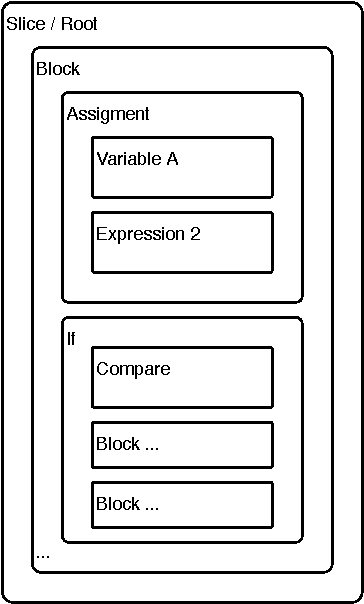
\includegraphics[width=.8\linewidth]{figures/representation.pdf}
    \caption{Our internal slice representation.}
    \label{fig:representation}
\end{figure}

We represent vulnerabilities, that we pretend to discover, as objects as well. We parsed them from the 
second JSON argument to an object. If the file has three vulnerabilities, for instance, we would create
three objects. We search for vulnerabilities one by one, this allows to detect and resolve ambiguities.
For example, suppose that we have two vulnerabilities when the same function name X, has different types.
In the first vulnerability X is a sink, and on the second X is a source. This could lead to ambiguities.
See Section \ref{sec:efficiency} for detailed explanation.

Since an uninitialized variable is considered a source, we need a way to identify which variables were
initialized. We built a table, designed by Symbol Table (Abr: SymTable, denoted by $\mathcal{S}$) which 
saves every variable found during the parsing and object construction.
Whenever we find a variable, we checked if it already exists on SymTable. If it was new we contruct a
new \textsc{Variable} object and added it to the SymTable. Otherwise SymTable just return the object.
This allows to have only one object per variable and use it multiple times by its reference.

\subsection*{Explicit Flows}
%explain how we use a symtable
In order to detect explicit flow we need a way to link sources and sinks through assigments.
We know that only variables can be sources and function calls can be either sources, sanitizers or sinks.
Then every \textsc{Variable} and \textsc{FunctionCall} has now a type, which can be one of the three. It is now trivial
to identify if a given \textsc{FunctionCall} is a source, for instance, because we can check its type which is a
property of \textsc{FunctionCall} objects.

However if we assign a source \textsc{FunctionCall} F to a \textsc{Variable} A, then A it is not a source
but has a source which is F. We need a way to propagate this information back to A.
We design a change to our \textsc{Variable} and \textsc{FunctionCall} objects, which saves a list of source,
sanitizers and sinks. For instance, suppose the following example:

\begin{lstlisting}[language=Python]
a = 2
a = source()
\end{lstlisting}

After the first assigment, the sources (denoted by $Src_X$) of A will be empty.
After the second assigment, the sources of A will be the sources of the right value of the assigment.
$X = Y \rightarrow Src_X = Src_Y$

The object \textsc{FunctionCall} \textit{source} has it self as a source since it is defined that
way in the vulnerability pattern file. $Src_{source} = source$
Then it is trivial to see that sources of \textit{a} will be the sources of \textit{source} $Src_a = source$

Now consider the case where we have a non source function, say \textit{func} which as several uninitialized
variables as arguments:

\begin{lstlisting}[language=Python]
a = func(b, c, d)
\end{lstlisting}

The sources of \textit{func} will be the union of sources of arguments in that function.
Intuitively, $Src_{func(arg_1, arg_2, ..., arg_n)} = Src_{arg_1} \cup Src_{arg_2} \cup ... \cup Src_{arg_n} = \bigcup_{arg_i}^{arg_n} Src_{arg_i} $
This applies for every other object structures, like \textsc{BinaryOperation}, etc and the logic is the
same for sanitizers.

Now consider an example where there are multiple branches:

\begin{lstlisting}[language=Python]
a = source()
if True:
    a = source2()
else:
    a = source3()

sink(a)
\end{lstlisting}

Whenever we detect a new block, which happens when there are indentation, we create a copy of the current SymTable
to the block, so we can later merge changes.

For example, previous examples contains two blocks, one for the if body and another one for the else body.
Before the \textsc{If} instruction, $\mathcal{S} = <a>$ $Src_a = source$
After the \textsc{If} instruction both if and else blocks SymTable will have $a$ but the source is different.
$a \in \mathcal{S}_{If}: Src_a = source2$ $a \in \mathcal{S}_{Else}: Src_a = source3$
Then we union both SymTable and replace the current SymTable with the result. $\mathcal{S} = \mathcal{S}_{If} \cup \mathcal{S}_{Else} $

$(a \in \mathcal{S}_{If}: Src_a = source2) \cup (a \in \mathcal{S}_{Else}: Src_a = source3) = a \in \mathcal{S}: Src_a = source2, source3$

Next, we replace the current SymTable with the result of the previous union operation. $Src_a = source$ become
$Src_a = source2, source3$.

If \textsc{Else} body is ommited we perform the exactly same logic. \textsc{Else} receives a copy of the SymTable
which will not change since there are no instructions in that block ($\mathcal{S}_{Else} = \mathcal{S}$). When merge occur, it will merge the \textsc{If}
SymTable with a copy of the current context.
$(a \in \mathcal{S}_{If}: Src_a = source2) \cup (a \in \mathcal{S}_{Else}: Src_a = source) = a \in \mathcal{S}: Src_a = source, source2$

The same logic is applied for inners \textsc{If} and for \textsc{While} and for \textsc{ElsIf} which are no more than
another \textsc{If} inside the \textsc{Else}.

\subsection*{Efficiency}
\label{sec:efficiency}
Our internal structure allow us to perform every check for each vulnerability pattern only one time, i.e.
if we have one vulnerability in the pattern file, we built and traverse our internal representation once only!
We add support for visitors to traverse the slice and perform additional logic. However we were able to
to detected vulnerabilities on the fly as the matryoska is being constructed, without need a second traverse.

However if we have more than one vulnerability we built and traverse our internal representation for each
vulnerability, i.e. we search for vulnerability one by one. Unfortunately we did not have time but we pretend
to optimize allowing to search all vulnerabilities at once. We would need to change our internal structure to store 
sources, sanitizers and sinks for a list of vulnerabilities. This could introduce bugs that we would not have
time to test but we pretended to do.

\subsection*{Implicit Flows}
%explain what we do to check implicit flows, like propagate the sources of a condition to every assigment
%in the body